\documentclass[12pt, a4paper, oneside]{ctexart}
\usepackage{amsmath, amsthm, amssymb, bm, color, framed, graphicx, hyperref, mathrsfs,diagbox,amsfonts, amssymb}
\graphicspath{ {./images/} }
\title{\textbf{《随机过程》第二次作业 }} 
\author{24 2022010910017 谢卿云}
\date{\today}
\linespread{1.5}
\definecolor{shadecolor}{RGB}{241, 241, 255}
\newcounter{problemname}
\newenvironment{problem}{\begin{shaded}\stepcounter{problemname}\par\noindent\textbf{题目\arabic{problemname}. }}{\end{shaded}\par}
\newenvironment{solution}{\par\noindent\textbf{解答. }}{\par}
\newenvironment{note}{\par\noindent\textbf{题目\arabic{problemname}的注记. }}{\par}

\begin{document}
	
	\maketitle
	
	\begin{problem}
		设随机过程 $\{X(t),-\infty<t<+\infty\}=\{X(t, \omega),-\infty<t<+\infty\}$ 只有两条样本函数.
		\[X\left(t, \omega_{1}\right)=2 \cos (t), X\left(t, \omega_{2}\right)=-2 \cos (t),\]
		且 $P\left(\omega_{1}\right)=\frac{2}{3}, P\left(\omega_{2}\right)=\frac{1}{3}$. 求:(1)一维分布函数 $F_{0}(x)$ 和 $F_{\pi / 4}(x)$;(2)二维分布函数 $F_{0, \pi / 4}(x, y)$;(3)均值函数 $\mu_{X}(t)$; (3) 协方差函数 $\gamma_{X}(s, t)$.
		
	\end{problem}
	
	\begin{solution}\\
		(1)分别代入$t=0, \frac{\pi}{4}$得到\\
		\[F_0(x)=\begin{cases}
			1&,x\ge 2\\
			\frac{1}{3}&,-2\le x <2\\
			0&,x<-2
		\end{cases}\]
		\[F_{\pi /4 }(x)=\begin{cases}
			1&,x\ge \sqrt{2}\\
			\frac{1}{3}&,-\sqrt{2}\le x <2\\
			0&,x<-\sqrt{2}\\
		\end{cases}\]
		(2)注意到$F_{0, \pi / 4}(x, y)=F_0(x)F_{\pi /4}(y)$.
		\[F_{0, \pi / 4}(x, y)=\begin{cases}
			1&,x\ge 1,y\ge 1\\
			\frac{1}{3}&,x\ge 2,-\sqrt{2}\le y<\sqrt{2}or -2\le x<2,y\ge \sqrt{2}\\
			\frac{1}{9}&,-\sqrt{2}\le y<\sqrt{2},-2\le x<2\\
			0&,else.
		\end{cases}\]
		(3)$\mu_X(t)=E(X(t))=2cos(t)\times \frac{2}{3} - 2cos(t)\times \frac{1}{3}=\frac{2}{3}cos(t)$\\
		(4)$\gamma_X(s,t)=E[X(s)X(t)]-E[X(s)]E[X(t)]=[\frac{4}{9}\cdot 2cos(s)\cdot 2cos(t) - \frac{2}{9}\cdot 2cos(s)\cdot 2cos(t) - \frac{2}{9}\cdot 2cos(s)\cdot 2cos(t)+\frac{1}{9}\cdot 2cos(s)\cdot 2cos(t)] -\frac{2}{3}cos(s)\frac{2}{3}cos(t)=0$
	\end{solution}
	
%	\begin{note}
%		这里是注记. 
%	\end{note}

	\begin{problem}
		考虑正弦波过程 $\{X(t)=\xi \cos (\omega t) | t \geq 0\}$, 其中 $\omega$ 为正常数, $\xi \sim U[0,1]$. 求: (1) 分别求 $t=\frac{\pi}{4 \omega}, \frac{\pi}{2 \omega}, \frac{3 \pi}{4 \omega}, \frac{\pi}{\omega}$ 时 $X(t)$ 概率密度函数 $f_{t}(x)$; (2) 求 $X(t)$ 的均值函数, 方差函数, 自相关函数,协方差函数。
		
	\end{problem}
	\begin{solution}\\
		(1)$X(\frac{\pi}{4 \omega})=\frac{\xi}{\sqrt{2}},f_{\pi/4\omega}(x)=\begin{cases}\sqrt{2}&,0\le x\le \frac{1}{\sqrt2}\\ 0&,else\end{cases}$\\
		$X(\frac{\pi}{2 \omega})=0,f_{\pi/3\omega}(x)=\delta(0)$,也就是在$x=0$处的Dirac-$\delta$函数.\\
		$X(\frac{3\pi}{4 \omega})=-\frac{\xi}{\sqrt{2}},f_{3\pi/4\omega}(x)=\begin{cases}\sqrt{2}&,-\frac{1}{\sqrt2}\le x\le 0 \\ 0&,else\end{cases}$\\
		$X(\frac{\pi}{ \omega})=-\xi,f_{\pi/\omega}(x)=\begin{cases}1&,-1\le x\le 0 \\ 0&,else\end{cases}$\\
		(2)$\mu_X(t)=E[X(t)]=\int_{0}^{1}\xi cos(\omega t)d\xi=\frac{1}{2}cos(\omega t)$\\
		$E[X^2(t)]=\int_{0}^{1}\xi^2 cos^2(\omega t)d\xi=\frac{1}{3}cos^2(\omega t)$\\
		$D[X(t)]=E[X^2(t)]-E^2(X(t))=\frac{1}{12}cos^2(\omega t)$\\
		$R(s,t)=E[X(s)X(t)]=\int_{0}^{1}\xi^2 cos(\omega t)cos(\omega s)d\xi=\frac{1}{3}cos(\omega s)cos(\omega t)$\\
		$R\gamma(s,t)=E[X(s)X(t)]-E[X(s)]E[X(t)]==\frac{1}{12}cos(\omega s)cos(\omega t)$\\
	\end{solution}
	
	\begin{problem}
		考虑随机游走模型 $\{Y(n), n=0,1,2, \cdots\}$,其中
		$$
		Y(n)=\sum_{k=1}^{n} X_{k}, Y(0)=0
		$$
		$X_{k}$ 是相互独立同服从 $N\left(0, \sigma^{2}\right)$ 的正态随机变量。求:(1) $Y(n)$ 的概率密度;
		
		(2) $(Y(n), Y(m))$ 的联合概率密度 $(m \geq n)$.
	\end{problem}
	
	\begin{solution}\\
		(1)注意到$\psi_Y(t)=E(e^{ity})=E(e^{it\sum_{i=1}^{n}X_i})=\prod_{i=1}^{n}E(e^{itX_k})=e^{-\frac{1}{2}n\sigma^2t}$,\\
		因此$Y\sim N(0,n\sigma^2),f_Y(y)=\frac{1}{\sigma \sqrt{2\pi n}} e^{-\frac{y^2}{2n\sigma^2} }$\\
		(2)对于$m>n$,$f_{(Y(n),Y(m))}=f_{Y(n)}(x)f_{Y(m)|Y(n)}(y|x)=\frac{1}{\sigma \sqrt{2\pi n}}e^{-\frac{x^2}{2n\sigma^2}}\frac{1}{\sigma \sqrt{2\pi (m-n)}}e^{-\frac{(y-x)^2}{2(n-m)\sigma^2}}$\\
		对于$m=n$,$f_{(Y(n),Y(m))}=f_{Y(n)}(x)f_{Y(m)|Y(n)}(y|x)=\begin{cases}
			\frac{1}{\sigma \sqrt{2\pi n }}e^{-\frac{x^2}{2n\sigma^2}}&,y=x\\
				0&,else.
		\end{cases}$\\
	\end{solution}
	
	
	\begin{problem}
		一个通讯系统, 以每 $T$ 秒为一周期输出一个幅度为 $A$ 的信号, $A$ 为常数, 每个周期内信号输出时间 $X_{i} \sim U\left[0, \frac{5}{6} T\right]$, 持续时间 $Z_{i} \sim U\left[0, \frac{1}{6} T\right], X_{i}, Z_{i}$ 相互独立, 且输出时间 $X_{i}$ 相互独立, 持续时间 $Z_{i}$ 也相互独立, 如下图所示, 设 $Y(t)$ 为 $t$ 时刻接收到的信号幅度, 求 $\{Y(t), t \geq 0\}$ 的一维概率分布。
	\end{problem}
	
	\begin{center}
		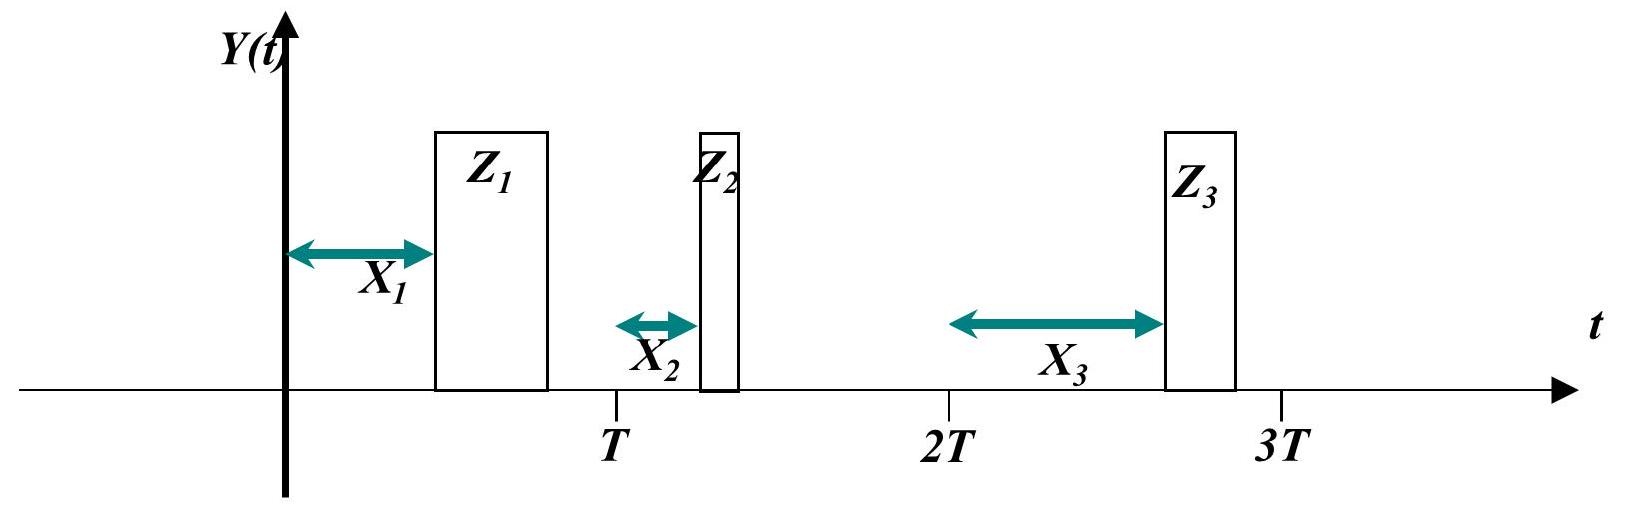
\includegraphics[width=\textwidth]{2024_03_21_329fdc051168c33e87b9g-1}
	\end{center}
	
	\begin{solution}
		注意到令$R=X_i+Z_i$,$R$的概率密度为$f_R(r)=\int_{-infty}^{\infty}f_X(x)f_Z(r-x)dx$,也就是\\
		$$
		f_R(r)=\begin{cases}
			0&,r\le 0\\
			\frac{36r}{5T^2}&,0<r\le \frac{1}{6}T\\
			\frac{6}{5T}&,\frac{1}{6}T<r\le \frac{5}{6}T\\
			\frac{36}{5T^2}(T-r)&,\frac{5}{6}T<r<T\\
			0&,r\ge T
		\end{cases}
		$$		
		那么R的分布$F_R(u)=\int_{-\infty}^{u}f_R(r)dr$\\
		$$
			F_R(u)=\begin{cases}
				0&,u\le 0\\
				\frac{18u^2}{5T^2}&,0<u\le \frac{1}{6}T\\
				\frac{6u}{5T}-\frac{1}{10}&,\frac{1}{6}T<u<\frac{5}{6}T\\
				-\frac{13}{5}+\frac{36}{5T^2}(Tu-\frac{1}{2}u^2),&\frac{5}{6}\le u<T\\
				1&,u\ge T
			\end{cases}
		$$
		记$\delta = \{\frac{t}{T}\}T$,则因为每个周期相互独立,只需要考虑一个周期内的情况\\
		$$
		P({Y(t)=0})=P({\delta< X_i})+P({\delta>X_i+Z_i})
		$$
		$$
		=\begin{cases}
			1-\frac{6\delta}{5T}&,0<\delta <\frac{5}{6}T\\
			0&,\delta>\frac{5}{6}T
		\end{cases}+
		\begin{cases}
			\frac{18\delta ^2}{5T^2}&,0<\delta \le \frac{1}{6}T\\
			\frac{6\delta }{5T}-\frac{1}{10}&,\frac{1}{6}T<\delta <\frac{5}{6}T\\
			-\frac{13}{5}+\frac{36}{5T^2}(T\delta -\frac{1}{2}\delta ^2),&\frac{5}{6}T\le \delta <T\\
		\end{cases}$$
		$$
		=\begin{cases}
			1-\frac{6\delta}{5T}+\frac{18\delta ^2}{5T^2}&,0<\delta \le \frac{1}{6}T\\
			\frac{9}{10}&,\frac{1}{6}T<\delta <\frac{5}{6}T\\
			-\frac{13}{5}+\frac{36}{5T^2}(T\delta -\frac{1}{2}\delta ^2),&\frac{5}{6}T\le \delta <T\\
		\end{cases}
		$$
		显然$P({Y(t)=A})=1-P({Y(t)=0})$,这里不再赘述.
	\end{solution}
	
	\begin{problem}
		通过连续重复抛郑一枚硬币确定随机过程 $\{X(t), t \geq 0\}$.
		$$
		X(t)= \begin{cases}\cos (\pi t), & \text { 在 } t \text { 时刻抛掷硬币出现正面 } \\ 2 , & \text { 在 } t \text { 时刻抛郑硬币出现反面 }\end{cases}
		$$
		
		求:(1)一维分布函数 $F_{1 / 2}(x)$ 和 $F_{t}(x)$; (2) 二维分布函数 $F_{1 / 2,1}(x, y)$;
	\end{problem}
	\begin{solution}\\
		(1)由于硬币均匀,所以以下结论是平凡的:
		$$
		F_{t}(x)=\begin{cases}
			0&,x<cos\pi t\\
			\frac{1}{2}&,cos\pi t\le x\le 2\\
			1&,x\ge 2
		\end{cases}
		$$
		代入$t=\frac{1}{2}$,我们有\\
		$$
		F_{\frac{1}{2}}(x)=\begin{cases}
			0&,x<0\\
			\frac{1}{2}&,0 \le x\le 2\\
			1&,x\ge 2
		\end{cases}
		$$
		(2)我们默认不同时间投掷硬币的试验是相互独立的,$X(\frac{1}{2}),X(1)$的联合分布如下表所示,\\
		\begin{table}[h]
			\centering
			\caption{联合分布率}\label{tab:tab2} 
			
				\begin{tabular}{|c|c|c|}
				\hline
				\diagbox{$X(\frac{1}{2})$}{$X(1)$}&-1&2 \\ 
				\hline
				0&$\frac{1}{4}$&$\frac{1}{4}$\\ 
				\hline
				2&$\frac{1}{4}$&$\frac{1}{4}$\\ 
				\hline
				\end{tabular} 
			
		\end{table}\\
		不难得出分布函数如下所示\\
		$$
		F_{\frac{1}{2},1}(x,y)=\begin{cases}
			\frac{1}{4}&,0<x<2,-1<y<2\\
			\frac{1}{2}&,0<x<2,y\ge 2\ or x\ge2,-1<y<2\\
			1&,x\ge 2,y\ge2\\
			0&,else.
		\end{cases}
		$$
	\end{solution}
	\begin{problem}
		设 $X(t)=\sin (\Theta t)$, 其中 $\Theta \sim U[0,2 \pi]$, 证明: (1) $\{X(t), t=0,1,2, \ldots\}$ 是宽平稳序列;(2)而 $\{X(t), t \geq 0, \ldots\}$ 不是宽平稳过程。
	\end{problem}
	\begin{solution}\\
		(1)注意到$E(X(t))=\int_{0}^{2\pi} sin(\theta t)\frac{1}{2\pi} d\theta = \frac{1}{2\pi t}cos(u)|_0^{2\pi t}$,当$t\in \mathbb{Z},E(X(t))=0$为常数;\\
		$\gamma(t,s)=E(X(s)X(t))=E(sin(\theta s)sin(\theta t))$\\$=\int_{0}^{2\pi }sin(\theta s)sin(\theta t)\frac{1}{2\pi}d\theta =\begin{cases}0&,s\neq t\\ \frac{1}{2}&,s=t\end{cases}$只和$t-s$有关,故$\{X(t), t=0,1,2, \ldots\}$ 是宽平稳序列.\\
		(2)$E(X(t))=\int_{0}^{2\pi} sin(\theta t)\frac{1}{2\pi} d\theta = \frac{1}{2\pi t}cos(u)|_0^{2\pi t}$,对$t\ge 0$不为常数,故$\{X(t), t \geq 0, \ldots\}$ 不是宽平稳过程.
	\end{solution}
	
	\begin{problem}
		设二阶矩过程 $\{X(t),-\infty<t<+\infty\}$ 有均值函数 $\mu_{X}(t)=\alpha+\beta t$, 协方差函数 $\gamma_{X}(s, t)=$ $e^{-\lambda|t-s|}$, 令$$Y(t)=X(t+1)-X(t)$$\\
		证明 $\{Y(t),-\infty<t<+\infty\}$ 为宽平稳过程。
	\end{problem}
	\begin{solution}
		 $\mu_Y(t)=E[X(t+1)-X(t)]=E[X(t+1)]-E[(X(t))]$\\
		 $=\alpha+\beta(t+1)-\alpha-\beta t=\beta$为常数\\
		 注意到$E[X(s)X(t)]=e^{-\lambda|t-s|}+(\alpha+\beta s)(\alpha +\beta t)$\\
		 故$\gamma_Y(s,t)=E[Y(s)Y(t)]-E[Y(s)]E[Y(t)]=E[X(s+1)X(t+1)]+E[X(s)X(t)]-E[X(s+1)X(t)]-E[X(s)X(t+1)]-\beta^2=\gamma_X(s+1,t+1)+\gamma_X(s,t)-\gamma_X(s+1,t)-\gamma_X(s,t+1)$只与$|t-s|$有关,因此$\{Y(t),-\infty<t<+\infty\}$ 为宽平稳过程.
	\end{solution}
	
	
	\begin{problem}
		设随机过程 $\{X(t)=\xi \cos (\beta t+\eta),-\infty<t<+\infty\}$, 其中 $\xi \sim N(0,1), \eta \sim U[0,2 \pi]$, $\xi$ 与 $\eta$ 相互独立, $\beta$ 为正常数, 证明 $\{X(t),-\infty<t<+\infty\}$ 为宽平稳过程, 且均值具有遍历性。
	\end{problem}
	\begin{solution}
		只需验证以下三点即可:\\
		(1)$E[X(t)]=E(\xi cos(\beta t +\eta))=E(\xi)E(cos(\beta t+\eta))=0$为常数\\
		(2)
		$$\gamma_X(s,t)=E[X(s)X(t)]=\frac{1}{2}(E^2(\xi)+D(\xi))(E[cos(\beta(s-t))]+E[cos(\beta(s+t)+2\eta)])$$$$=\frac{1}{2}cos(\beta(t-s))+\int_{0}^{2\pi}cos[\beta(s+t)+2\eta]\frac{1}{2\pi}=\frac{1}{2}cos(\beta(s-t))$$
		只与s-t有关, 改记$\gamma(\tau)=\frac{1}{2}cos(\beta \tau)$.\\
		(3)$$\lim_{T\to +\infty}\frac{1}{T}\int_{0}^{2T}(1-\frac{\tau}{2T})\gamma(\tau)d\tau=\lim_{T\to +\infty}\frac{1}{2T\beta} \left(  \frac{sin\beta \tau(2T-\tau)}{2T}-\frac{1}{2T}\frac{cos\beta \tau}{\beta} \right)\big|_{0}^{2T}=0$$
		因此均值遍历性定理可知结论为真.
	\end{solution}
	
	\begin{problem}
		设随机过程 $\{X(t)=A \cos (\omega t+\Theta),-\infty<t<+\infty\}$, 其中 $A, \omega, \Theta$ 为相互独立的随机变量。 $E(A)=2, D(A)=4, E\left(A^{4}\right)=8$, 且 $\omega \sim U[-5,5], \Theta \sim U[-\pi, \pi]$. 令 $Z(t)=$ $X(t) X(t+u)$ 这里 $u>0$ 为常数。讨论 $\{Z(t),-\infty<t<+\infty\}$ 的宽平稳性和均值遍历性。
	\end{problem}
	\begin{solution}
		$E[X(t)]=E(A)E[cos(\omega t + \theta)]=2\int_{-\pi}^{\pi}\int_{-5}^{5}cos(\omega t+\theta)=0$\\
		$\gamma(s,t)=E[X(s)X(t)]=E[A^2cos(\omega t +\theta)cos(\omega s+ \theta)]=4\int_{-5}^{5}cos(\omega(t-s))\frac{1}{10}d\omega+4\int_{-5}^{5}\int_{-\pi}^{\pi}cos(\omega(t+s)+2\theta)\frac{1}{2\pi}\frac{1}{10}d\theta d\omega=\frac{4}{5(t-s)}sin5(t-s)$
		因此$\mu_Z(t)=E[X(t)X(t+u)]=\frac{4sinu}{5u}$\\
		$$R_Z(s,t)=E[X(s)X(t)X(s+u)X(t+u)]$$$$=E(A^4)E[cos(\omega t +\theta)cos(\omega s +\theta)cos(\omega (s+u) +\theta)cos(\omega (t+u) +\theta)]$$$$=2E[cos(\omega (s+t)+2\theta)]+2E[cos^2((\omega(s-t)))]
		=1+\frac{sin(10(s-t))}{10(s-t)}+\frac{sin10u}{10u}$$
		$$\gamma_Z(s,t)=R_Z(s,t)-\mu_Z^2(t)=1+\frac{sin(10(s-t))}{10(s-t)}+\frac{sin10u}{10u}-\frac{16}{sin^2(5u)}{25u^2}$$
		期望为常数,协方差函数只和$s-t$有关,故$\{Z(t),-\infty<t<+\infty\}$ 具有宽平稳性.\\
		但$\lim_{T\to +\infty}\frac{1}{T}\int_{0}^{2T}(1-\frac{\tau}{2T})\gamma(\tau)d\tau=1+\frac{sin(10u)}{10u}-\frac{16sin5u}{25u^2}$不一定为0,故不一定具备均值遍历性.
	\end{solution}
	
	\begin{problem}
		若 $Z_{0}, Z_{1}, \cdots$ 是独立同分布随机变量, 定义 $X_{n}=Z_{0}+Z_{1}+\cdots+Z_{n}$, 证明 $\left\{X_{n}, n=\right.$ $0,1,2, \cdots\}$ 是平稳独立增量过程。
	\end{problem}
	\begin{solution}\\
		(1)独立性:注意到$X(n)-X(n-1)=Z(n)$,因为$Z_{0}, Z_{1}, \cdots$ 是独立同分布,显然$X(n)$也是独立增量过程.\\
		(2)平稳性:注意到$\psi_{X(n)}(a)=E(e^{ia\sum_{i=0}^{n}Z_i})=\psi_Z^n(t)$
			显然$\psi_{X(s+t)}(a)=\psi_{X(s)}(a)\psi_{X(t)}(a)$,由平稳增量定理可知$X(n)$也是平稳的.
	\end{solution}
\end{document}
